%!TEX root = main.tex

\chapter{Numerical Approximation for Unconstrained Optimization}\label{chapter:UnconstrainedNumerical}
Although technically any characterization result finds the exact value of the extrema of a function, computationally this is hardly feasible (specially for functions of very high dimension).  See the following session based on problem \ref{problem:tricky} for an example, where we try to find the critical points of the function $f(x,y,z)=e^{x^2+y^2+z^2}-x^4-y^y-z^6$ symbolically in Python with the \texttt{sympy} libraries:

% framesep=2mm,
% baselinestretch=1.2,
\begin{minted}[frame=single, fontsize=\footnotesize, linenos ]{python}
# Importing necessary symbols/libraries/functions
from sympy.abc import x,y,z
from sympy import Matrix, solve, exp
from sympy.tensor.array import derive_by_array

# Description of f, computation of its gradient and Hessian
f = exp(x**2 + y**2 + z**2) - x**4 -y**6 - z**6
gradient = derive_by_array(f, [x,y,z])
hessian  = Matrix([derive_by_array(gradient, a) for a in [x,y,z]])
\end{minted}
While the correct expressions for $\gradient{f}$ and $\Hess{f}$ are quickly computed, trying to find critical points results in an error:
\begin{minted}[frame=single,fontsize=\footnotesize,mathescape]{python}
>>> solve(gradient) # Search of critical points by solving $\gradient{f}=0$
NotImplementedError: could not solve 
4*x**2*sqrt(-log(exp(x**2)/(2*x**2))) - 6*(-log(exp(x**2)/(2*x**2)))**(5/2)
\end{minted}

Too complex a task to be performed symbolically, although the obvious answer is $(0,0,0)$.  A better way to approach this is by trying to approximate this minimum using the structure of the graph of $f$.  In these notes we are going to explore several strategies to accomplish this task, based on the concept of \emph{iterative methods for finding zeros of real-valued functions}.

%!TEX root = notes.tex

\section{Newton's Method}
\begin{example}[The Newton-Raphson method]
In order to find a good estimation of $\sqrt{2}$ with mani decimal places, we allow a computer to find better and better approximations of the solution of the equation $f(x)=x^2-2$.  We start with an initial guess, say $x_0=3$.  We construct a sequence $\{ x_n \}_{n\in\field{N}}$ that converges to $\sqrt{2}$ as follows:
\begin{enumerate}
\item Find the tangent line to the graph of $f$ at $x_0$, 
\begin{equation*}
y-f(x_0)=f'(x_0)(x-x_0)
\end{equation*}
\item Provided this line is not horizontal ($f'(x_0)\neq 0$), report the intersection of this line with the $x$--axis.  Call this intersection $x_1$
\begin{equation*}
x_1=x_0-\frac{f(x_0)}{f'(x_0)}
\end{equation*}
\item Repeat this process, to get the sequence 
\begin{equation*}
x_{n+1} = x_n - \frac{f(x_n)}{f'(x_n)}
\end{equation*}
\end{enumerate}
\begin{figure}[ht!]
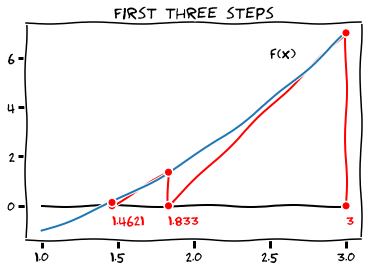
\includegraphics[width=0.65\linewidth]{newton1.png}
\caption{Newton-Raphson iterative method}
\label{figure:Newton-Raphson}
\end{figure}
Note the result of applying this process a few times:

\begin{table}[ht!]
\begin{tabular}{|c|c|r|} \hline 
$n$ & $x_n$ & $f(x_n)$ \\ \hline \hline 
$0$ & $3.000000000000000$ & $7.0000E+00$ \\ \hline 
$1$ & $1.833333333333333$ & $1.3611E+00$ \\ \hline 
$2$ & $1.462121212121212$ & $1.3780E-01$ \\ \hline 
$3$ & $1.414998429894803$ & $2.2206E-03$ \\ \hline 
$4$ & $1.414213780047198$ & $6.1568E-07$ \\ \hline 
$5$ & $1.414213562373112$ & $4.7518E-14$ \\ \hline 
$6$ & $1.414213562373095$ & $-4.4409E-16$ \\ \hline 
$7$ & $1.414213562373095$ & $4.4409E-16$ \\ \hline 
\end{tabular}
\caption{Convergence to $\sqrt{2}$ with 15-digit accuracy in 6 steps}
\label{table:Newton-Raphson}
\end{table}
\end{example}

\begin{example}\label{example:NewtonRaphsonChoice}
Consider now the function $f(x) = 1-\tfrac{1}{x}$ over $(0, \infty)$, which has the obvious root $x=1$. The Newton-Raphson method gives the following iterates for any $x_0 \in (0,\infty)$:
\begin{align*}
x_{n+1} = x_n - \frac{f(x_n)}{f'(x_n)} = x_n \big( 2- x_n \big).
\end{align*}
Notice the two factors in the right-hand side of that expression: $x_n$, and $2-x_n$.  If the initial guess does not satisfy $0<x_0<2$, then the next iteration gives a non-positive value (see Figure \ref{figure:NewtonRaphsonChoice}).  The method will not work on those instances: convergence to a solution is not guaranteed.
\begin{figure}[ht!]
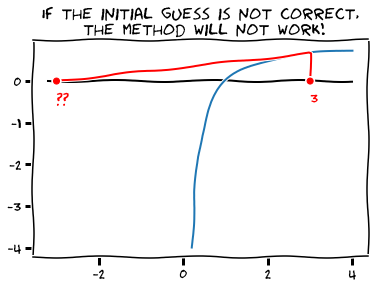
\includegraphics[width=0.65\linewidth]{badNewton.png}
\caption{Initial guess must carefully be chosen in Newton-Raphson}
\label{figure:NewtonRaphsonChoice}
\end{figure}
\end{example}

\begin{example}\label{example:NewtonRaphsonloop}
Consider now $f(x) = \sign(x)\sqrt{\lvert x \rvert}$ over $\field{R}$, with root at $x=0$.  The Newton-Raphson method fails miserably with this function: for any $x_0 \neq 0$
\begin{align*}
x_1 = x_0 - \frac{f(x_0)}{f'(x_0)} = x_0 - \frac{\sign(x_0)\lvert x_0 \rvert^{1/2}}{\tfrac{1}{2}\lvert x_0 \rvert^{-1/2}} = -x_0.
\end{align*}
This sequence turns into a loop: $x_{2n}=x_0$, $x_{2n+1}=-x_0$ for all $n\in \field{N}$ (see Figure \ref{figure:NewtonRaphsonloop}).
\begin{figure}[ht!]
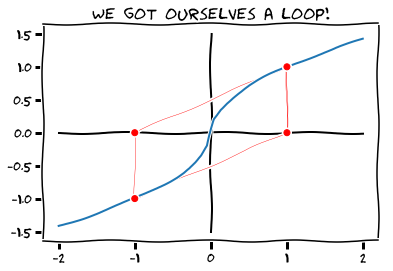
\includegraphics[width=0.65\linewidth]{loop.png}
\caption{Newton-Raphson fails for some functions}
\label{figure:NewtonRaphsonloop}
\end{figure}
\end{example}

Let's proceed to extend this process to functions $\boldsymbol{g} \colon \field{R}^d \to \field{R}^d$ as follows.  
\begin{itemize}
	\item Any function $\boldsymbol{g} \colon \field{R}^d \to \field{R}^d$ can be described in the form $\boldsymbol{g}(\x) = \big[ g_1(\x), g_2(\x), \dotsc, g_d(\x) \big]$ for $d$ real-valued functions $g_k\colon \field{R}^d \to \field{R}$ ($1\leq k \leq d$).
	\item For such a function $\boldsymbol{g}$, we may express its gradient as a $d\times d$ matrix in the form
	\begin{equation*}
	\gradient{\boldsymbol{g}} = \begin{bmatrix}
	\frac{\partial g_1}{\partial x_1} & \frac{\partial g_1}{\partial x_2} & \dotsb & \frac{\partial g_1}{\partial x_d} \\ \\
	\frac{\partial g_2}{\partial x_1} & \frac{\partial g_2}{\partial x_2} & \dotsb & \frac{\partial g_2}{\partial x_d} \\ \\
	\vdots & \vdots & \ddots & \vdots \\ \\
	\frac{\partial g_d}{\partial x_1} & \frac{\partial g_d}{\partial x_2} & \dotsb & \frac{\partial g_d}{\partial x_d} \\
	\end{bmatrix}
	\end{equation*}
\end{itemize}
Start with a guess for the solution, $\x_0$, and on the $n$--th step of the algorithm compute the $(n+1)$--th term of the sequence by
\begin{equation}\label{equation:NewtonMethod}
\x_{n+1} = \x_n - \big[ \gradient{\boldsymbol{g}}(\x_n) \big]^{-1} \boldsymbol{g}(\x_n),
\end{equation}
where $\big[ \gradient{\boldsymbol{g}}(\x_n) \big]^{-1}$ represents the inverse matrix of the gradient at $\x_n$.  This is equivalent to selecting in the tangent hyperplane to the graph of $\boldsymbol{g}$ at $\boldsymbol{g}(\x_n)$, the one line in the direction with the most rapid increase/decrease.  The computation of $\x_{n+1}$ is therefore the intersection of that line with the hyperplane $x_d=0$.  We refer to $\big[ \gradient{\boldsymbol{g}}(\x_n) \big]^{-1} \boldsymbol{g}(\x_n)$ as the \emph{Newton direction} for $\boldsymbol{g}$ at $\x_n$.

\begin{example}\label{example:preNewton4poly4}
Consider the function $\boldsymbol{g}\colon \field{R}^2 \to \field{R}^2$ given by
\begin{equation*}
\boldsymbol{g}(x,y,z) = \big[ x^3-y, y^3-x \big]
\end{equation*}
Its gradient at each $(x,y)$ is given by
\begin{equation*}
\gradient{\boldsymbol{g}}(x,y) = \begin{bmatrix} 3x^2 & -1 \\ -1 & 3y^2 \end{bmatrix}
\end{equation*}
Note the determinant of this matrix is $\det \gradient{\boldsymbol{g}}(x,y) = 9x^2y^2-1 = (3xy-1)(3xy+1)$.  For any point $(x,y)$ that does not make this expression zero, this is an invertible matrix with 
\begin{equation*}
\big[ \gradient{\boldsymbol{g}}(x,y)\big]^{-1} = \frac{1}{9x^2y^2-1}\begin{bmatrix} 3y^2 & 1 \\ 1 & 3x^2 \end{bmatrix}
\end{equation*}
For an initial guess $(x_0, y_0)$, the sequence computed by the Newton method is then given by
\begin{align*}
\begin{bmatrix} x_{n+1} \\ y_{n+1} \end{bmatrix} &= \begin{bmatrix} x_n \\ y_n \end{bmatrix} -\frac{1}{9 x_n^2 y_n^2-1}\begin{bmatrix} 3y_n^2 & 1 \\ 1 & 3x_n^2 \end{bmatrix} \begin{bmatrix} x_n^3-y_n \\ y_n^3-x_n \end{bmatrix} \\
% &= \begin{bmatrix}
% x_n - \frac{3x_n^3 y_n^2-2 y_n^3-x_n}{9x_n^2  y_n^2-1} \\  y_n - \frac{3x_n^2 y_n^3+-2x_n^3- y_n}{9x_n^2 y_n^2-1}
% \end{bmatrix}
\end{align*}
Let's run this process with three different initial guesses:
\begin{enumerate}
	\item Starting at $(x_0, y_0) = (-1.0,1.0)$, the sequence converges to $(0,0)$.  %See Table \ref{table:00}.
	\begin{table}[ht!]
	\begin{tabular}{|c|c|c|} \hline 
	$n$ & $x_n$ & $y_n$ \\ \hline \hline 
	$0$ & $-1.00000000$ & $1.00000000$ \\ \hline 
	$1$ & $-0.50000000$ & $0.50000000$ \\ \hline 
	$2$ & $-0.14285714$ & $0.14285714$ \\ \hline 
	$3$ & $-0.00549451$ & $0.00549451$ \\ \hline 
	$4$ & $-0.00000033$ & $0.00000033$ \\ \hline 
	$5$ & $-0.00000000$ & $0.00000000$ \\ \hline 
	$6$ & $-0.00000000$ & $0.00000000$ \\ \hline 
	\end{tabular}
	\caption{Convergence to $(0,0)$ with 8-digit accuracy in 5 steps}
	\label{table:00}
	\end{table}
	\item Starting at $(x_0,y_0) = (3.5, 2.1)$, the sequence converges to $(1,1)$.  %See Table \ref{table:11}.
	\begin{table}[ht!]
	\begin{tabular}{|c|c|c|} \hline 
	$n$ & $x_n$ & $y_n$ \\ \hline \hline 
	$0$ & $3.50000000$ & $2.10000000$ \\ \hline 
	$1$ & $2.37631607$ & $1.57961573$ \\ \hline 
	$2$ & $1.65945969$ & $1.27476534$ \\ \hline 
	$3$ & $1.23996276$ & $1.10419072$ \\ \hline 
	$4$ & $1.04837462$ & $1.02274752$ \\ \hline 
	$5$ & $1.00260153$ & $1.00133122$ \\ \hline 
	$6$ & $1.00000824$ & $1.00000451$ \\ \hline 
	$7$ & $1.00000000$ & $1.00000000$ \\ \hline 
	$8$ & $1.00000000$ & $1.00000000$ \\ \hline 
	\end{tabular}
	\caption{Convergence to $(1,1)$ with 8-digit accuracy in 7 steps}
	\label{table:11}
	\end{table}
	\item Starting at $(x_0, y_0) = (-13.5, -7.3)$, the sequence converges to $(-1,-1)$.  %See Table \ref{table:-1-1}.
	\begin{table}[ht!]
	\begin{tabular}{|c|c|c|} \hline 
	$n$ & $x_n$ & $y_n$ \\ \hline \hline 
	$0$ & $-13.50000000$ & $-7.30000000$ \\ \hline 
	$1$ & $-9.00900415$ & $-4.92301873$ \\ \hline 
	$2$ & $-6.01982204$ & $-3.36480659$ \\ \hline 
	$3$ & $-4.03494126$ & $-2.36199873$ \\ \hline 
	$4$ & $-2.72553474$ & $-1.73750959$ \\ \hline 
	$5$ & $-1.87830623$ & $-1.36573112$ \\ \hline 
	$6$ & $-1.36121191$ & $-1.15374930$ \\ \hline 
	\end{tabular}
	\begin{tabular}{|c|c|c|} \hline 
	$n$ & $x_n$ & $y_n$ \\ \hline \hline 
	$7$ & $-1.09518303$ & $-1.04341362$ \\ \hline 
	$8$ & $-1.00932090$ & $-1.00463507$ \\ \hline 
	$9$ & $-1.00010404$ & $-1.00005571$ \\ \hline 
	$10$ & $-1.00000001$ & $-1.00000001$ \\ \hline 
	$11$ & $-1.00000000$ & $-1.00000000$ \\ \hline 
	$12$ & $-1.00000000$ & $-1.00000000$ \\ \hline 
	$13$ & $-1.00000000$ & $-1.00000000$ \\ \hline 
	\end{tabular}
	\caption{Convergence to $(-1,-1)$ with 8-digit accuracy in 11 steps}
	\label{table:-1-1}
	\end{table}
\end{enumerate}
\end{example}

We can readily see how this process aids in the computation of critical points of twice continuously differentiable real-valued function $f\colon \field{R}^d \to \field{R}$:
\begin{enumerate}
	\item Set $\boldsymbol{g}(\x) = \gradient{f}(\x) = \big[ \frac{\partial f}{\partial x_1}, \dotsc, \frac{\partial f}{\partial x_d} \big]$
	\item It is then $\gradient{\boldsymbol{g}}(\x) = \Hess{f}(\x)$
	\item Perform a Newton method (with initial guess $\x_0$) on $\boldsymbol{g}=\gradient{f}$ to obtain the recurrence formula
	\begin{equation}\label{equation:Newton4Crit}
	\x_{n+1} = \x_n - \big[ \Hess{f}(\x_n) \big]^{-1} \cdot \gradient{f}(\x_n)
	\end{equation}
\end{enumerate}

\begin{example}
Consider the polynomial $p_4(x,y) = x^4-4xy+y^4$. Notice $\gradient{p_4}(x,y) = \big[ x^3-y, y^3-x \big]$---this is function $\boldsymbol{g}$ in Example \ref{example:preNewton4poly4}.  The critical points we found were $(0,0)$, $(-1,-1)$ and $(1,1)$.  See Figure \ref{figure:NewtonConvergence}.
\end{example}
\begin{example}
A similar process for the Rosenbrock function 
\begin{equation*}
\mathcal{R}_{1,1}(x,y) = (1-x)^2 + (y-x^2)^2
\end{equation*}
gives the following recurrence formula:
\begin{align*}
\begin{bmatrix} x_{n+1} \\ y_{n+1} \end{bmatrix} &=
\begin{bmatrix} x_{n} \\ y_{n} \end{bmatrix} - \big[ \Hess{\mathcal{R}_{1,1}}(x_n,y_n) \big]^{-1} \cdot \gradient{\mathcal{R}_{1,1}}(x_n, y_n) \\
% &= \begin{bmatrix} x_{n} \\ y_{n} \end{bmatrix} - \tfrac{2}{2x^2-2y+1} \begin{bmatrix}
% 1/2 & x_n \\ x_n & 6x_n^2-2y_n+1
% \end{bmatrix} \begin{bmatrix}
% 2x_n^3-2x_n y_n +x_n -1 \\ y_n -x_n^2
% \end{bmatrix} \\
&= \frac{1}{2x_n^2-2y_n+1} \begin{bmatrix}
2x_n^3-2x_n y_n+1 \\ x_n(2x_n^3-2x_n y_n-x_n+2)
\end{bmatrix}
\end{align*}
For instance, starting with the initial guess $(x_0, y_0) = (-2,2)$, the sequence converges to the critical point $(1,1)$.  See Figure \ref{figure:NewtonConvergence}.
\end{example}
\begin{figure}[ht!]
\begin{tabular}{cc}
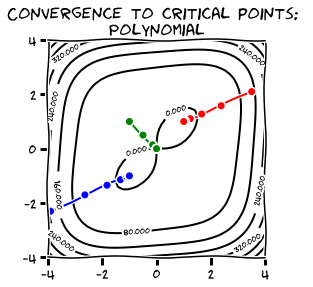
\includegraphics[width=0.45\linewidth]{convergenceNewton.png} &
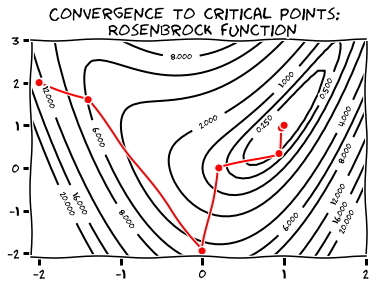
\includegraphics[width=0.55\linewidth]{convergenceNewtonRosenbrock.png} 
\end{tabular}
\caption{Newton method}
\label{figure:NewtonConvergence}
\end{figure}

\begin{remark}
Newton's Method to solve $\boldsymbol{g}=\boldsymbol{0}$, as given by the recurrence formula in equation \eqref{equation:NewtonMethod} in page \pageref{equation:NewtonMethod}, is very convenient to provide explicit descriptions of the different iterations.  However, it is hardly suitable for practical purposes, due to the computational issues involving matrix inversion.

To avoid dealing with matrix inversion, we consider the following equivalent formula:
\begin{equation}
\gradient{\boldsymbol{g}}(\x_n) \cdot \big( \x_{n+1} - \x_n \big) = -\boldsymbol{g}(\x_n)
\end{equation}
This is a simple system of linear equations, and thus much faster to solve.  

The equivalent recurrence formula to search for critical points of a twice continuously differentiable real-valued function $f \colon \field{R}^d \to \field{R}$ is thus
\begin{equation}
\Hess{f}(\x_n) \cdot (\x_{n+1}-\x_n) = -\gradient{f}(\x_n).
\end{equation}
\end{remark}

\begin{example}
The equivalent recurrence formula to the one we obtained in example \ref{example:preNewton4poly4} is as follows:
\begin{equation*}
\begin{bmatrix} 3x_n^2 & -1 \\ -1 & 3y_n^2 \end{bmatrix} \begin{bmatrix} x_{n+1}-x_n \\ y_{n+1}-y_n \end{bmatrix} = \begin{bmatrix} x_n^3 - y_n \\ y_n^3 - x_n \end{bmatrix}
\end{equation*}
All we need to do is, at each step $n$, solve for $X$ and $Y$ the system of linear equations
\begin{equation*}
\begin{cases}
3x_n^2 (X-x_n) - (Y-y_n)  = x_n^3 - y_n \\
-(X-x_n) + 3y_n^2 (Y-y_n) = y_n^2 - x_n
\end{cases}
\end{equation*}
or equivalently,
\begin{equation*}
\begin{cases}
3x_n^2 X - Y = 4x_n^3 - 2y_n \\
-X + 3y_n^2 Y = 4y_n^2 - 2x_n
\end{cases}
\end{equation*}
\end{example}

There are some theoretical results that aid in the search for a \emph{good} initial guess.  The following states a simple set of conditions on $f$ and $\x_0$ to guarantee \emph{quadratic convergence}\footnote{See Appendix \ref{appendix:convergence}} of the corresponding sequences $\{ \x_n \}_{n \in \field{N}}$ to a critical point $\xstar$.

\begin{theorem}[Quadratic Convergence Theorem]\label{theorem:QuadraticConvergence}
Suppose $f\colon \field{R}^d \to \field{R}$ is a twice continuously differentiable real-valued function, and $\xstar$ is a critical point of $f$. Let $\mathcal{N}(\x) = \x - \big[ \Hess{f}(\x) \big]^{-1} \cdot \gradient{f}(\x)$. If there exists 
\begin{enumerate}
	\item $h>0$ so that\footnote{Recall the \emph{norm} of a matrix $M$, defined by $\norm{M} = \max\{ \norm{M\cdot \x} : \norm{\x}=1 \}$.} $\big\lVert \big[ \Hess{f}(\xstar)\big]^{-1} \big\rVert \leq \tfrac{1}{h}$,
	\item $\beta>0$, $L>0$ for which $\norm{\Hess{f}(\x) - \Hess{f}(\xstar)} \leq L \norm{ \x - \xstar }$ provided $\norm{ \x - \xstar }\leq \beta$.
\end{enumerate}
In that case, for all $\x \in \field{R}^d$ satisfying $\norm{ \x - \xstar }\leq \min \{\beta, \tfrac{2h}{3L} \}$,
\begin{equation*}
\frac{\norm{ \mathcal{N}(\x) - \xstar }}{\norm{\x - \xstar}^2} \leq \frac{3L}{2h}
\end{equation*}
\end{theorem}

\begin{example}
Consider the function $f(x)=x-\log x$ on $(0,\infty)$, which has a global minimum at $x^\star=1$.  Its gradient is $f'(x)=1-\tfrac{1}{x}$, the function we studied in Example \ref{example:NewtonRaphsonChoice} in page \pageref{example:NewtonRaphsonChoice}.  We did establish then any initial guess $x_0$ should belong in the interval $(0,2)$.  We want to use Theorem \ref{theorem:QuadraticConvergence} to improve the search, so we may guarantee \emph{quadratic convergence} to the critical point.  
\begin{itemize}
	\item The Hessian is $f''(x)=x^{-2}$, and thus $\big\lVert \big[ \Hess{f}(x^\star) \big]^{-1} \big\rVert = 1$. 
	\item Notice that for all $0<x<2$,
	\begin{equation*}
	\norm{\Hess{f}(x) - \Hess{f}(x^\star)} = \big\lvert \tfrac{1}{x^2}  - 1 \big\rvert =\frac{1+x}{x^2}\abs{x-1}
	\end{equation*}
	Choosing e.g.~$\beta=\tfrac{1}{2}$, we readily obtain that $\frac{10}{9} \leq \frac{1+x}{x^2}\leq 6$;
	therefore, $\norm{\Hess{f}(x) - \Hess{f}(x^\star)} \leq 6 \abs{x-1}$, and we may choose $L=6$ for $\beta=\tfrac{1}{2}$.
\end{itemize}
Theorem \ref{theorem:QuadraticConvergence} guarantees that any initial guess $\x_0 \in \big(\tfrac{8}{9}, \tfrac{10}{9}\big)$ will give us good results.  

\begin{figure}[ht!]
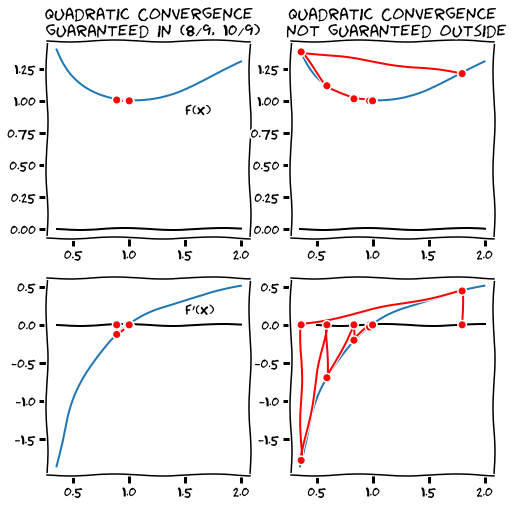
\includegraphics[width=0.75\linewidth]{quadraticConv.png}
\caption{Quadratic Convergence of the Newton-Raphson method}
\label{figure:QuadraticConvergence}
\end{figure}
\end{example}
%!TEX root = main.tex

\section{The Method of Steepest Descent}\index{Steepest descent}\index{Gradient!descent|see {Steepest descent}}

The method of \emph{Steepest Descent} (also known as the method of \emph{Gradient Descent}) is based upon the following property of gradients that we learned in Vector Calculus:

\begin{theorem}
If $f \colon \field{R}^d \to \field{R}$ is continuously differentiable, then at any point $\x \in \field{R}^d$, the vector $-\gradient{f}(\x)$ points in the direction of most rapid decrease for $f$ at $\x$.  The rate of decrease of $f$ at $\x$ in this direction is precisely $-\norm{\gradient{f}(\x)}$.
\end{theorem}

\begin{remark}\index{Steepest descent!direction of}\index{Direction!of steepest descent}
For this reason, the vector $-\gradient{f}(\x)/\norm{\gradient{f}(\x)}$ is called the \emph{direction of steepest descent} of $f$ at $\x$.
\end{remark}

\separator

In order to search for a local minimum for a twice continuously differentiable function $f\colon \field{R}^d \to \field{R}$, we start by choosing an initial guess $\x_0$.  
\begin{enumerate}
	\item Restrict the function $f$ over the line through $\x_0$ in the direction of $-\gradient{f}(\x_0)$:
	\begin{equation*}
	\varphi_0(t) = f\big( \x_0 - t \gradient{f}(\x_0) \big), \quad t\geq 0
	\end{equation*}
	\item \emph{Line-search}: Search for the value of $t_0 \geq 0$ that minimizes $\varphi_0$, and set\index{Line-search}
	\begin{equation*}
	\x_1 = \x_0 - t_0\gradient{f}(\x_0)
	\end{equation*}
	\item Repeat this process to get the sequence
	\begin{gather}\label{equation:SteepestDescent}
	\begin{split}
	&\x_{n+1} = \x_n - t_n \gradient{f}(\x_n), \\ &t_n = \argmin_{t\geq 0} \varphi_n(t) = \argmin_{t\geq 0} f\big(\x_n - t\gradient{f}(\x_n)\big)
	\end{split}
	\end{gather}
\end{enumerate}

\begin{remark}\index{Steepest descent!sequence of}
Sequences constructed following the formula in \eqref{equation:SteepestDescent} are said to be \emph{sequences of Steepest Descent} for $f$.

Unlike Newton-Raphson or the secant methods, this algorithm guarantees that these sequences are non-increasing: $f(\x_{n+1}) \leq f(\x_n)$ for all $n \in \field{N}$.  And even better: if there is convergence, their limit must be a critical point of $f$.  These results are formalized in Theorems \ref{theorem:SteepestDescentDescends} and \ref{theorem:SteepestDescentConvergesToCritical}  below.

Steepest descent sequences have another interesting property: on each step $n$, the direction of steepest descent is perpendicular to the direction of steepest descent of step $n+1$ (!!)  We state and prove this result in Theorem \ref{theorem:SteepestDescentPerpSteps}.
\end{remark}

\begin{theorem}\label{theorem:SteepestDescentDescends}
Let $f\colon \field{R}^d \to \field{R}$ be a continuously differentiable real-valued function, and let $\{ \x_n \}_{n\in\field{N}}$ be a sequence of steepest descent for $f$.  If $\gradient{f}(\x_N) \neq 0$, then $f(\x_{N+1}) < f(\x_N)$.
\end{theorem}

\begin{theorem}\label{theorem:SteepestDescentConvergesToCritical}
Let $f\colon \field{R}^d \to \field{R}$ be a real-valued function, let $\x_0 \in \field{R}^d$ be an initial guess.  Assume $S = \{ \x \in \field{R}^d :  f(\x) \leq f(\x_0) \}$ is a compact set and $f$ is continuously differentiable in $S$.  Under these conditions, the limit of any convergent subsequence of the associated sequence of steepest descent $\{ \x_n \}_{n\in \field{N}}$ is a critical point of $f$.
\end{theorem}

\begin{theorem}\label{theorem:SteepestDescentPerpSteps}
Let $f \colon \field{R}^d \to \field{R}$ be a continuously differentiable real-valued function, and $\{ \x_n \}_{n\in\field{N}}$ a sequence of steepest descent for $f$.  For any $n \in \field{N}$, $\langle \x_{n+2} - \x_{n+1}, \x_{n+1} - \x_n \rangle = 0$.
\end{theorem}
\begin{proof}
Consider for each $n \in \field{N}$ the function $\varphi_n(t) = f\big(\x_n -t \gradient{f}(\x_x)\big)$, with a global minimum at $t_n \geq 0$.  It must then be
\begin{equation*}
0 = \varphi_n'(t_n) = \langle \gradient{f}(\x_n), -\gradient{f}\big( \x_n - t_n \gradient{f}(\x_n)\big) \rangle = - \langle \gradient{f}(\x_{n+1}), \gradient{f}(\x_n) \rangle,
\end{equation*}
which proves that the gradient of consecutive terms of the sequence of steepest descent for $f$ are perpendicular.  Now, by virtue of the recurrence formula \eqref{equation:SteepestDescent},
\begin{align*}
\langle \x_{n+2} - \x_{n+1}, &\,\x_{n+1} - \x_n \rangle = \langle t_{n+1}\gradient{f}(\x_{n+1}), t_n \gradient{f}(\x_n) \rangle \\
&= t_{n+1}t_n \langle \gradient{f}(\x_{n+1}), \gradient{f}(\x_n) \rangle = 0, 
\end{align*}
which proves the statement.
\end{proof}

\begin{example}
For the polynomial function $p_4(x,y) = x^4-4xy+y^4$ from Example \ref{example:NewtonPoly4}, using the same initial guesses as in Example \ref{example:preNewton4poly4}, we find the following behavior:
\begin{itemize}
	\item Starting at $(x_0, y_0) = (-1.0,1.0)$, the sequence jumps to $(0,0)$ in one step.  At that point, since the gradient of the function is zero, the method of Steepest descent ceases to work.
	% \begin{table}[ht!]
	\begin{center}
	\begin{tabular}{|r|r|r|r|} \hline 
	$n$ & $x_n$ & $y_n$ & $f(x_n,y_n)$ \\ \hline \hline 
	$0$ & $-1.000000$ & $1.000000$ & $6.000000$ \\ \hline 
	$1$ & $0.000000$ & $0.000000$ & $0.000000$ \\ \hline 
	$2$ & \texttt{nan} & \texttt{nan} & \texttt{nan} \\ \hline 
	\end{tabular}
	% \caption{Steepest Descent: Convergence to $(0,0)$ accurately in exactly one step.}
	% \label{table:SD00}
	% \end{table}
	\end{center}
	\item Starting at $(x_0,y_0) = (3.5, 2.1)$, the sequence converges to $(1,1)$.
	% \begin{table}[ht!]
	\begin{center}
	\begin{tabular}{|r|r|r|r|} \hline 
	$n$ & $x_n$ & $y_n$ & $f(x_n,y_n)$ \\ \hline \hline 
	$0$ & $3.500000$ & $2.100000$ & $140.110600$ \\ \hline 
	$1$ & $1.044472$ & $1.753064$ & $3.310777$ \\ \hline 
	$2$ & $1.141931$ & $1.063276$ & $-1.878163$ \\ \hline 
	$3$ & $1.008581$ & $1.044435$ & $-1.988879$ \\ \hline 
	$4$ & $1.013966$ & $1.006319$ & $-1.998931$ \\ \hline 
	$5$ & $1.000898$ & $1.004472$ & $-1.999891$ \\ \hline 
	$6$ & $1.001437$ & $1.000651$ & $-1.999989$ \\ \hline 
	$7$ & $1.000093$ & $1.000461$ & $-1.999999$ \\ \hline 
	% \end{tabular}~\begin{tabular}{|r|r|r|r|} \hline 
	% $n$ & $x_n$ & $y_n$ & $f(x_n,y_n)$ \\ \hline \hline 
	$8$ & $1.000149$ & $1.000067$ & $-2.000000$ \\ \hline 
	$9$ & $1.000010$ & $1.000048$ & $-2.000000$ \\ \hline 
	$10$ & $1.000015$ & $1.000007$ & $-2.000000$ \\ \hline 
	$11$ & $1.000001$ & $1.000005$ & $-2.000000$ \\ \hline 
	$12$ & $1.000002$ & $1.000001$ & $-2.000000$ \\ \hline 
	$13$ & $1.000000$ & $1.000001$ & $-2.000000$ \\ \hline 
	$14$ & $1.000000$ & $1.000000$ & $-2.000000$ \\ \hline 
	$15$ & $1.000000$ & $1.000000$ & $-2.000000$ \\ \hline 
	\end{tabular}
	% \caption{Steepest Descent: Convergence to $(1,1)$ with 6-digit accuracy in 13 steps.}
	% \label{table:SD11}
	% \end{table}
	\end{center}
	\item Starting at $(x_0, y_0) = (-13.5, -7.3)$, the sequence converges to $(1,1)$ as well.
	% \begin{table}[ht!]
	\begin{center}
	\begin{tabular}{|r|r|r|r|} \hline 
	$n$ & $x_n$ & $y_n$ & $f(x_n,y_n)$ \\ \hline \hline 
	$0$ & $-13.500000$ & $-7.300000$ & $35660.686600$ \\ \hline 
	$1$ & $2.362722$ & $-4.871733$ & $640.498302$ \\ \hline 
	$2$ & $1.434154$ & $1.194162$ & $-0.586492$ \\ \hline 
	$3$ & $1.021502$ & $1.130993$ & $-1.896212$ \\ \hline 
	$4$ & $1.038817$ & $1.017881$ & $-1.991558$ \\ \hline 
	$5$ & $1.002305$ & $1.012291$ & $-1.999167$ \\ \hline 
	$6$ & $1.003909$ & $1.001808$ & $-1.999917$ \\ \hline 
	$7$ & $1.000236$ & $1.001246$ & $-1.999992$ \\ \hline 
	% \end{tabular}~\begin{tabular}{|r|r|r|r|} \hline 
	% $n$ & $x_n$ & $y_n$ & $f(x_n,y_n)$ \\ \hline \hline 
	$8$ & $1.000399$ & $1.000185$ & $-1.999999$ \\ \hline 
	$9$ & $1.000024$ & $1.000127$ & $-2.000000$ \\ \hline 
	$10$ & $1.000041$ & $1.000019$ & $-2.000000$ \\ \hline 
	$11$ & $1.000002$ & $1.000013$ & $-2.000000$ \\ \hline 
	$12$ & $1.000004$ & $1.000002$ & $-2.000000$ \\ \hline 
	$13$ & $1.000000$ & $1.000001$ & $-2.000000$ \\ \hline 
	$14$ & $1.000000$ & $1.000000$ & $-2.000000$ \\ \hline 
	$15$ & $1.000000$ & $1.000000$ & $-2.000000$ \\ \hline 
	\end{tabular}
	% \caption{Steepest Descent: Convergence to $(1,1)$ with 6-digit accuracy in 14 steps.}
	% \label{table:SD-1-1}
	% \end{table}
	\end{center}
\end{itemize}
\begin{figure}[ht!]
% \begin{tabular}{c}
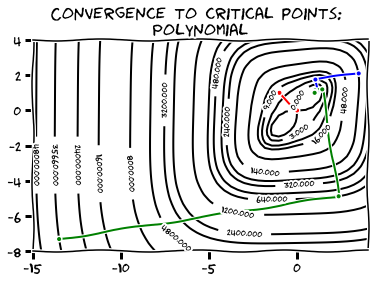
\includegraphics[width=0.7\linewidth]{images/convergenceSteepest.png}
% 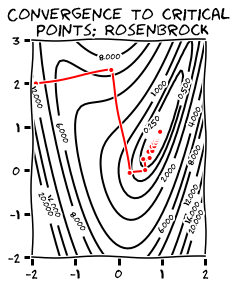
\includegraphics[width=0.65\linewidth]{images/SDR3.png}
% \end{tabular}
\caption{The Method of Steepest Descent: Polynomial function}
\label{figure:SteepestConvergenceP}
\end{figure}
\end{example}

\begin{example}\label{example:SDR}\index{Function!Rosenbrock}
Notice what happens when we try to implement the same process on the Rosenbrock function $\mathcal{R}_{1,1}(x,y) = (1-x)^2 + (y-x^2)^2$, with the initial guess $(x_0, y_0) = (-2,2)$.  The sequence does converge to the minimum $(1,1)$, albeit very slowly.
\begin{center}
\begin{tabular}{|r|r|r|r|} \hline 
 $n$ & $x_n$ & $y_n$ & $f(x_n,y_n)$ \\ \hline \hline 
$0$ & $-2.000000$ & $2.000000$ & $13.000000$ \\ \hline 
$1$ & $-0.166290$ & $2.309522$ & $6.567163$ \\ \hline 
$2$ & $0.256054$ & $-0.056128$ & $0.568264$ \\ \hline 
$3$ & $0.613477$ & $0.007683$ & $0.285318$ \\ \hline 
$4$ & $0.568566$ & $0.259241$ & $0.190235$ \\ \hline 
$5$ & $0.715784$ & $0.285524$ & $0.132227$ \\ \hline 
$6$ & $0.689755$ & $0.431319$ & $0.098227$ \\ \hline 
$7$ & $0.779264$ & $0.447299$ & $0.074310$ \\ \hline 
$8$ & $0.761554$ & $0.546496$ & $0.057977$ \\ \hline 
$9$ & $0.823325$ & $0.557524$ & $0.045696$ \\ \hline 
$10$ & $0.810322$ & $0.630358$ & $0.036667$ \\ \hline 
$11$ & $0.855862$ & $0.638488$ & $0.029614$ \\ \hline 
$12$ & $0.845883$ & $0.694385$ & $0.024199$ \\ \hline 
$13$ & $0.880846$ & $0.700627$ & $0.019862$ \\ \hline 
$14$ & $0.872964$ & $0.744776$ & $0.016437$ \\ \hline 
$15$ & $0.900551$ & $0.749702$ & $0.013647$ \\ \hline 
$16$ & $0.894200$ & $0.785276$ & $0.011399$ \\ \hline 
\end{tabular}~\begin{tabular}{|r|r|r|r|} \hline
 $n$ & $x_n$ & $y_n$ & $f(x_n,y_n)$ \\ \hline \hline 
$17$ & $0.916394$ & $0.789239$ & $0.009544$ \\ \hline 
$18$ & $0.911201$ & $0.818326$ & $0.008028$ \\ \hline 
$19$ & $0.929317$ & $0.821560$ & $0.006766$ \\ \hline 
$20$ & $0.925024$ & $0.845608$ & $0.005723$ \\ \hline 
$21$ & $0.939976$ & $0.848277$ & $0.004847$ \\ \hline 
$22$ & $0.936397$ & $0.868329$ & $0.004118$ \\ \hline 
$23$ & $0.948845$ & $0.870551$ & $0.003502$ \\ \hline 
$24$ & $0.945840$ & $0.887385$ & $0.002986$ \\ \hline 
$25$ & $0.956276$ & $0.889248$ & $0.002548$ \\ \hline 
$26$ & $0.953739$ & $0.903457$ & $0.002178$ \\ \hline 
$27$ & $0.962537$ & $0.905028$ & $0.001864$ \\ \hline 
$28$ & $0.960386$ & $0.917075$ & $0.001597$ \\ \hline 
$29$ & $0.967837$ & $0.918405$ & $0.001369$ \\ \hline 
$30$ & $0.966007$ & $0.928657$ & $0.001176$ \\ \hline 
$31$ & $0.972342$ & $0.929788$ & $0.001010$ \\ \hline 
$32$ & $0.970780$ & $0.938539$ & $0.000869$ \\ \hline 
$33$ & $0.976182$ & $0.939503$ & $0.000748$ \\ \hline 
\end{tabular}
\end{center}
\end{example}

\begin{figure}[ht!]
% \begin{tabular}{c}
% 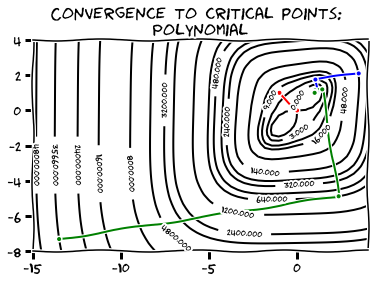
\includegraphics[width=0.65\linewidth]{images/convergenceSteepest.png} \\
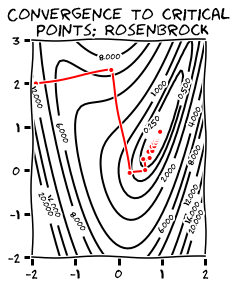
\includegraphics[width=0.6\linewidth]{images/SDR3.png}
% \end{tabular}
\caption{The Method of Steepest Descent: Rosenbrock Function}
\label{figure:SteepestConvergenceR}
\end{figure}

\subsection{Efficiency of Steepest Descent Method}

The analysis of efficiency of the method of Steepest descent is quite involved, but it boils down to studying the efficiency of Steepest descent for quadratic functions---since any function can be approximated using a Taylor's polynomial of degree two.  We will study that easier case in these notes.

\begin{theorem}[Taylor's Formula]\index{Theorem!Taylor's formula}
If $f\colon \field{R}^d \to \field{R}$ is a real-valued function of $d$ variables with continuous first and second partial derivatives on $\field{R}^d$, then for any choice $\x, \y \in \field{R}^d$, there exists a point $\boldsymbol{\xi} = \boldsymbol{\xi}(\x, \y)$ in the segment joining $\x$ and $\y$ so that
\begin{equation*}
f(\x) = f(\y) + \langle \gradient{f}(\y), \x - \y \rangle + \tfrac{1}{2} \quadratic{\Hess{f}(\boldsymbol{\xi})}(\x - \y)
\end{equation*}
\end{theorem}

\separator

Assume we have a quadratic function $p\colon \field{R}^d \to \field{R}$ satisfying $p(\boldsymbol{0}) = 0$.  There exist a $d$-dimensional vector $D = \big[q_1, \dotsc, q_d\big]$ and a symmetric matrix $Q = \big[ q_{jk} \big]_{j,k=1}^d$ (with $q_{jk}=q_{kj}$ for all $1\leq j,k \leq d$) so that
\begin{equation*}
p(\x) = \langle D, \x \rangle + \tfrac{1}{2}\quadratic{Q}(\x) = \sum_{k=1}^d \big( \tfrac{1}{2}q_{kk}x_k^2 + q_k x_k\big) + \sum_{1\leq j<k \leq d} q_{jk} x_j x_k
\end{equation*}
The gradient of this function is thus $\gradient{p}(\x) = x \cdot Q + D$.  It has one unique critical point $\xstar = -D Q^{-1}$ (Why?).  At that point, it is 
\begin{align}
p(\xstar) &= \tfrac{1}{2} \big( -D Q^{-1} \big)  Q \transpose{\big( -D Q^{-1} \big)} + D \transpose{\big( -D Q^{-1} \big)} \nonumber \\ 
&= \tfrac{1}{2} D Q^{-1} \transpose{D} - D Q^{-1} \transpose{D} \nonumber \\
&= -\tfrac{1}{2} D Q^{-1} \transpose{D} = -\tfrac{1}{2}\quadratic{(Q^{-1})}(D). \label{equation:pstarSD}
\end{align}
If $\x_n$ is a term in a sequence of steepest descent, then to compute $\x_{n+1}$ we proceed as follows:
\begin{enumerate}
	\item The direction of steepest descent at $\x_n$ is 
	\begin{equation*}\v_n = -\gradient{p}(\x_n) = -(x_n Q + D).
	\end{equation*}
	\item The restriction $\varphi\colon (0,\infty) \to \field{R}$ of the quadratic function $p$ over the half-line through $\x_n$ in the direction $\v_n$ is given by
	\begin{align*}
	\varphi(t) &= p( \x_n + t \v_n ) \\
	&= \tfrac{1}{2}(\x_n + t\v_n ) Q \transpose{(\x_n + t\v_n )} + D\transpose{(\x_n + t\v_n )} \\
	&= \tfrac{1}{2} \x_n Q \transpose{(\x_n + t\v_n )} + \tfrac{1}{2}t\v_n Q \transpose{(\x_n + t\v_n )} \\
	&\quad+D \transpose{\x}_n + tD \transpose{\v}_n \\
	&= \tfrac{1}{2}\x_n Q \transpose{\x}_n + \tfrac{1}{2} t\x_n Q \transpose{\v}_n + \tfrac{1}{2} t \v_n Q \transpose{\x}_n + \tfrac{1}{2} t^2 \v_n Q \transpose{\v}_n \\
	&\quad + D \transpose{\x}_n + t D \transpose{\v}_n \\
	&= \tfrac{1}{2} \underbrace{\v_n Q \transpose{\v}_n}_{\quadratic{Q}(\v_n)} t^2 + \underbrace{\tfrac{1}{2}\x_n Q \transpose{\x}_n + D \transpose{\x}_n}_{p(\x_n)} + tD\transpose{\v}_n + t \x_n Q \transpose{\v}_n \\
	&= \tfrac{1}{2} \quadratic{Q}(\v_n) t^2  + p(\x_n) + t \underbrace{\big( x_n Q + D \big)}_{-\v_n} \transpose{\v}_n \\
	&= \tfrac{1}{2}t^2 \v_n Q \transpose{\v}_n -  t \v_n \transpose{\v}_n + p(\x_n) \\
	&= \tfrac{1}{2} \quadratic{Q}(\v_n)t^2 - \norm{\v_n}^2 t + p(\x_n)
	\end{align*}
	\item The restriction function has its global minimum at
	\begin{equation*}
	t_n = \frac{\norm{\v_n}^2}{\quadratic{Q}(\v_n)};
	\end{equation*}
	therefore, the next iteration occurs at
	\begin{equation*}
	x_{n+1} = x_n + t_n \v_n = x_n + \frac{\norm{\v_n}^2}{\quadratic{Q}(\v_n)} \v_n 
	\end{equation*}
\end{enumerate}

\separator

We want to observe the convergence behavior of the sequence of evaluations $\{ p(\x_n) \}_{n \in \field{N}}$ to $p(\xstar)$.  We have
\begin{align*}
p(\x_{n+1}) &= p(\x_n + \tfrac{\norm{\v_n}^2}{\quadratic{Q}(\v_n)} \v_n) \\
&= \tfrac{1}{2} \quadratic{Q}(\v_n) \big( \tfrac{\norm{\v_n}^2}{\quadratic{Q}(\v_n)} \big)^2 - \norm{\v_n}^2 \tfrac{\norm{\v_n}^2}{\quadratic{Q}(\v_n)} + p(\x_n) \\
&= p(\x_n) - \frac{\norm{\v_n}^4}{2\quadratic{Q}(\v_n)}; 
\intertext{therefore,}
\frac{p(\x_{n+1}) - p(\xstar)}{p(\x_n)- p(\xstar)} &= \frac{p(\x_n) - p(\xstar) - \frac{\norm{\v_n}^4}{2\quadratic{Q}(\v_n)}}{p(\x_n) - p(\xstar)} \\
&= 1 - \frac{\norm{\v_n}^4}{ 2\quadratic{Q}(\v_n) \big( p(\x_n) - p(\xstar) \big)} \\
&= 1 - \frac{\norm{\v_n}^4}{2\quadratic{Q}(\v_n) \big( \tfrac{1}{2}\x_n Q \transpose{\x}_n + D \transpose{\x}_n + \tfrac{1}{2} DQ^{-1}\transpose{D} \big)} \\
&= 1 - \frac{\norm{\v_n}^4}{ \quadratic{Q}(\v_n) \big( \x_n Q \transpose{\x}_n+ 2D\transpose{\x}_n + DQ^{-1}\transpose{D} \big) }.
\end{align*}
Note in the denominator we may rewrite some of the terms:
\begin{align*}
\x_n Q \transpose{\x}_n &= \x_n Q (Q^{-1}Q) \transpose{\x}_n = (\x_n Q) Q^{-1} \transpose{(\x_n Q)}, \\
2D \transpose{\x}_n &= D\transpose{\x}_n + D\transpose{\x}_n = \x_n \transpose{D} + D (Q^{-1}Q) \transpose{\x}_n \\
&= \x_n (QQ^{-1}) \transpose{D} + D Q^{-1} \transpose{(\x_n Q)} \\
&= (\x_n Q) Q^{-1} \transpose{D} + D Q^{-1} \transpose{(\x_n Q)}.
\end{align*} 
This allows us to rewrite in the following convenient form 
\begin{align*}
\frac{p(\x_{n+1}) - p(\xstar)}{p(\x_n)- p(\xstar)} &= 1 - \frac{\norm{\v_n}^4}{ \quadratic{Q}(\v_n) (\x_n Q + D) Q^{-1} \transpose{(\x_nQ + D)} } \\
&= 1 - \frac{\norm{\v_n}^4}{\quadratic{Q}(\v_n) \quadratic{(Q^{-1})}(\v_n)}.
\end{align*}

We are ready to state the main result of this subsection:
\begin{theorem}\label{theorem:KantorovichEstimate}\index{Steepest descent!error}
Given a $d$-dimensional vector $D$, and a positive definite symmetric matrix $Q$ of size $d \times d$, consider the quadratic function $p(\x) = \tfrac{1}{2}\quadratic{Q}(\x) + \langle D , \x \rangle$.  Any sequence $\{ \x_n \}_{n \in \field{N}}$ of steepest descent converges to the global minimum $\xstar = -DQ^{-1}$.  The sequence of evaluations $\{ p(\x_n) \}_{n \in \field{N}}$ converges linearly to $p(\xstar) = -\tfrac{1}{2}\quadratic{(Q^{-1})}(D)$.  In particular, if $0 < \lambda_1 \leq \lambda_2 \leq \dotsb \leq \lambda_d$ are the eigenvalues of $Q$, then 
\begin{equation*}
\frac{p(\x_{n+1}) - p(\xstar)}{p(\x_n)- p(\xstar)} \leq \bigg( \frac{\lambda_d -\lambda_1}{\lambda_d + \lambda_1} \bigg)^2
\end{equation*}
\end{theorem}
\begin{proof}
We start by offering the following lower bound estimate\footnote{This is left as and advanced exercise. It is not too tricky; if you are stuck, see e.g.~\cite[section 1.3.1]{bertsekas1999nonlinear} for a proof.} involving the associated directions of steepest descent $\v_n$ in terms of the largest and smallest eigenvalues of $Q$.  For all $n \in \field{N}$,
\begin{equation}\label{equation:KantorovichEstimate}\index{Theorem!Kantorovich estimate}
\frac{\norm{\v_n}^4}{\quadratic{Q}(\v_n) \quadratic{(Q^{-1})}(\v_n)} \geq \frac{4\lambda_0\lambda_d}{(\lambda_0 + \lambda_d)^2}
\end{equation}
We have then
\begin{align*}
\frac{p(\x_{n+1}) - p(\xstar)}{p(\x_n)- p(\xstar)} &= 1 - \frac{\norm{\v_n}^4}{ \quadratic{Q}(\v_n) \quadratic{(Q^{-1})}(\v_n) } \\
&\leq 1 - \frac{4\lambda_1 \lambda_d}{(\lambda_1 + \lambda_d)^2} = \bigg( \frac{\lambda_d - \lambda_1}{\lambda_d + \lambda_1} \bigg)^2 \qedhere
\end{align*}
\end{proof}

\begin{example}\label{example:SDconvergenceRate}
The global minimum value of the quadratic function $p(x,y) = 5x^2 + 5y^2 -xy -11x +11y +11$ is zero, and found at $(1,-1)$.  Notice that we may write this function in the form $p(x,y) = \tfrac{1}{2}\quadratic{Q}(x,y) + \langle D, [x,y] \rangle + 11$, where
\begin{equation*}
D = [ -11, 11], \qquad Q = \begin{bmatrix} 10 & -1 \\ 10 & -1 \end{bmatrix}.
\end{equation*}
The symmetric matrix $Q$ has eigenvalues $\lambda_1 = 9 >0$, $\lambda_2 = 11 > 0$ and is therefore positive definite.  Theorem \ref{theorem:KantorovichEstimate} states that sequences of steepest descent exhibit linear convergence with a rate of convergence not larger than $\delta = \big( \tfrac{11-9}{11+9} \big)^2 = 0.01$.

Observe the computations of the first six iterations for values of the ratios $\frac{p(\x_n)}{p(\x_{n-1})}$ when we use $(1.5,3.5)$ as our initial guess.
\begin{center}
\begin{tabular}{|r|r|r|r|r|} \hline 
 $n$ & $x_n$ & $y_n$ & $p(x_n,y_n)$ & $\boldsymbol{\frac{p(x_n,y_n)}{p(x_{n-1},y_{n-1})}}$ \\ \hline \hline 
$0$ & $1.5000000000$ & $3.5000000000$ & $100.2500000000$ &  \\ \hline 
$1$ & $1.4498874016$ & $-0.9600212545$ & $1.0019989373$ & $\boldsymbol{0.0099950019}$ \\ \hline 
$2$ & $1.0049975009$ & $-0.9550224916$ & $0.0100149812$ & $\boldsymbol{0.0099950019}$ \\ \hline 
$3$ & $1.0044966254$ & $-0.9996004124$ & $0.0001000998$ & $\boldsymbol{0.0099950019}$ \\ \hline 
$4$ & $1.0000499500$ & $-0.9995504497$ & $0.0000010005$ & $\boldsymbol{0.0099950019}$ \\ \hline 
$5$ & $1.0000449438$ & $-0.9999960061$ & $0.0000000100$ & $\boldsymbol{0.0099950042}$ \\ \hline 
$6$ & $1.0000004993$ & $-0.9999955067$ & $0.0000000001$ & $\boldsymbol{0.0099950528}$ \\ \hline 
\end{tabular}
\end{center}
\end{example}

%!TEX root = main.tex

\section{Broyden's Secant Method}
Both Newton-Raphson and Steepest descent are sound methods, with their pros and their cons.  Steepest descent always converges to a local minimum, yet slowly.  Newton has a faster convergence, but we cannot always guarantee convergence.  Another drawback of both methods is the fact that we do need expressions for both the function itself and its derivative.  The \emph{Broydent Secant method} offers an improvement to some of these issues.

\subsection{A secant method to search for roots of univariate functions}
To explain how it works, let's once again try to find an accurate value of $\sqrt{2}$ as the root of the polynomial $p(x) = x^2-2$.
\begin{enumerate}
	\item Consider two initial guesses $x_0=3$, $x_1=2.8$.  Notice $f(3)= 7 \neq 5.84 = f(2.8)$.
	\item The line that joins the points $(3, 7)$ and $( 2,8, 5.84)$ has equation
	\begin{align*}
	y - 7 &= \frac{5.84-7}{2.8-3}(x-3), \\ 
	y &= 5.8x-10.4
	\end{align*}
	and intersects the $x$--axis at
	\begin{equation*}
	x_2 = \frac{10.4}{5.8} \approx 1.7931034483
	\end{equation*}
	\item Repeat this process to get a sequence $x_n$.
\end{enumerate}
\begin{example}
Observe the result of applying this recursive process, and compare with the similar experiment we conducted using the Newton-Raphson method in page \pageref{table:Newton-Raphson}.
\begin{center}
\begin{tabular}{|r|r|r|} \hline
$n$ & $x_n$ & $f(x_n)$ \\ \hline \hline
$0$ & $3.000000000000000$ & $7.0000E+00$ \\ \hline
$1$ & $2.800000000000000$ & $5.8400E+00$ \\ \hline
$2$ & $1.793103448275862$ & $1.2152E+00$ \\ \hline
$3$ & $1.528528528528528$ & $3.3640E-01$ \\ \hline
$4$ & $1.427253172054743$ & $3.7052E-02$ \\ \hline
$5$ & $1.414717869757887$ & $1.4267E-03$ \\ \hline
$6$ & $1.414215876250105$ & $6.5446E-06$ \\ \hline
$7$ & $1.414213562785585$ & $1.1667E-09$ \\ \hline
$8$ & $1.414213562373095$ & $8.8818E-16$ \\ \hline
\end{tabular}
\end{center}
\begin{figure}[ht!]
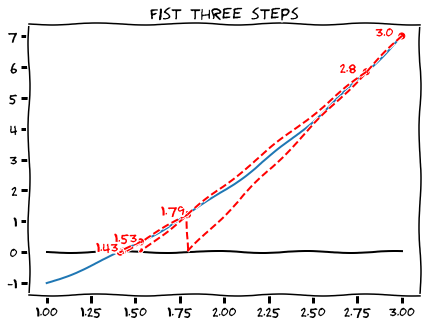
\includegraphics[width=0.6\linewidth]{images/secant.png}
\caption{Secant iterative method}\label{figure:SecantMethod}
\end{figure}
\end{example}

\begin{definition}\label{def:SecantMethod}\index{Secant method}\index{Secant method!iteration}\index{Secant method!recursive formula}
Given a function $f \colon \field{R} \to \field{R}$ and two initial guesses $x_0 \neq x_1$ satisfying $f(x_0) \neq f(x_1)$, we define the \emph{Secant method iteration} to be the sequence given by the following recursive formula
\begin{equation*}\label{equation:SecantMethod}\index{Secant method!iteration}
	x_{n+1} = x_{n-1} - \frac{x_n - x_{n-1}}{f(x_n) - f(x_{n-1})}f(x_{n-1})
\end{equation*}
The \emph{Secant method} refers to employing this sequence to search and approximate roots of the equation $f(x)=0$.
\end{definition}